\documentclass[a4paper,12pt]{article}
\usepackage[utf8]{inputenc}
\usepackage[T1]{fontenc}
\usepackage[left=2cm,right=2cm]{geometry}
\usepackage{graphicx}
\usepackage{wrapfig}
\usepackage{url}
\usepackage{amsmath}
\usepackage{amssymb}
\usepackage{titlesec}
\usepackage{titletoc}
\usepackage{lmodern}
\usepackage{microtype}

\begin{document}

\begin{center}
	
		\Large{Année universitaire 2019-2018}\\
		\Large{Université Toulouse Paul Sabatier}\\[1cm]
		
		\huge{Rapport de projet Modélisation et Calcul Scientifique}\\
		\vspace{3cm}
		
		Emma MAUGER\\
		Malalatiana RANDRIANARIJAONA
		
	\normalsize{\textit{ ~ M1 Développement Logiciel}}\\
		\medskip
		\vspace{2cm}
		
	\end{center}

\newpage
\tableofcontents
\pagenumbering{arabic}
\newpage

\section{myMFCCdistance}

Le premier TP consistait à programmer le calcul de la distance entre deux MFCC. Les MFCC étant des vecteurs de 13 valeurs, il nous fallait programmer la normalisation de ces deux vecteurs, qui se résume par la formule suivante : \emph{$\sqrt({\sum{x_i} - \sum{y_i})^2}$ avec i compris entre 1 et 13}.\\
Ensuite il a fallu programmer "norm", qui prend en paramètre un MFCC. Cette fonction renvoie simplement la valeur de mesure d'un MFCC, qui est son coefficient d'indice zéro. Cette valeur permet de déterminer si le MFCC correspond à un silence ou à un mot.
Puis, la fonction "unnoise", qui supprime le bruit (traduit par une MFCC) de la MFCC que l'on passe en paramètre. Pour ce faire, on soustrait à chaque coefficient de notre MFCC celui correspondant dans la MFCC traduisant le bruit. On retourne la nouvelle MFCC, épurée de tout bruit.

\section{myDTW}

Pour le calcul du Dynamic Time Warping (ou déformation temporelle dynamique) nous avons repris l'algorithme donné en TD. Nous avons donc créé une matrice de la taille des deux fields (deux ensembles de MFCC), plus un puisqu'il nous fallait ajouter une ligne et une colonne (les premières) ayant pour valeurs l'infini (traduit par MAX\_VALUE de java). La première "case" de la matrice devait être initialisée à zéro.
Ensuite, on calcule les DTW en conservant chaque calcul pour déterminer le minimum pour chaque case, entre les valeurs venant de gauche, de l'anti-diagonale supérieure et du haut. La dernière "case" de la matrice obtenue nous donne le score de cette DTW entre les deux ensembles de MFCC.

"ExtractFilesInFolder" est la fonction qui permet d'extraire les fichiers des dossiers.

Enfin, pour la fonction de la matrice de confusion, nous comparons les enregistrements d'une personne (test) avec d'autres enregistrements (référence). Les enregistrements dans le dossier référence sont triés par ordre alphabétique, pour que la différenciation entre les locuteurs soit plus aisée. Chacun des enregistrements du dossier test est comparé avec tous ceux du dossier référence, par locuteur. C'est-à-dire que pour 4 enregistrements de test différents ("alpha", "beta", "charlie" et "delta"), et pour deux locuteurs ("alpha\_1", "beta\_1", "charlie\_1", "delta\_1" et "alpha\_2", "beta\_2", "charlie\_2", "delta\_2"), on va comparer "alpha" du dossier test avec tous les "alpha\_i", "beta\_i", "charlie\_i", "delta\_i" du dossier référence, avec i allant de 1 au nombre de locuteur.
On initialise donc une matrice de la taille des deux fields avec toutes les valeurs à zéro. On calcule ensuite la différence entre les deux fields construits (un pour test, un pour référence), on conserve l'index de celui qui a la valeur minimale pour lui ajouter un dans la matrice de confusion. Dans un cas parfait, seule la diagonale aurait des valeurs différentes de zéro.
La somme des valeurs sur la diagonale de la matrice nous donne sa trace, à partir de laquelle on peut déterminer le taux de reconnaissance.

\begin{figure}[h]
		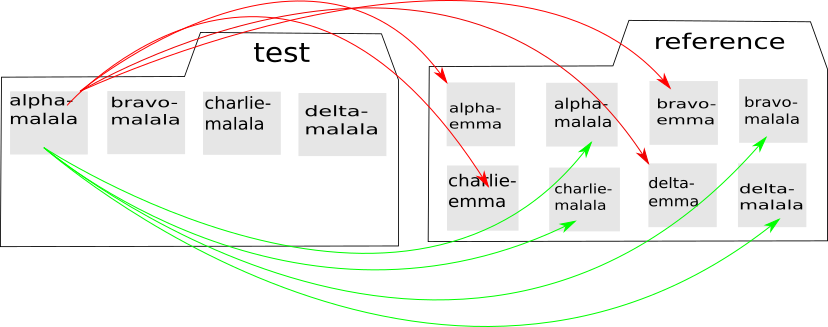
\includegraphics[scale=0.5]{compte-rendu.png}
	\end{figure}
	
\section{Résultats et analyse}
	//TODO dire qu'est ce qu'on cherche à faire ici
	\subsection{Test 1: Exemple simple sur enregistrement perso}
	\begin{table}[h]
		\begin{tabular}{|c|c|c|c|c|}
			\hline
			& alpha emma, malala & bravo emma, malala & charlie emma, malala & delta emma, malala\\
			\hline
			alpha-malala & 2 & 0 & 0 & 0 \\
			\hline
			bravo-malala & 1 & 1 & 0 & 0 \\
			\hline
			charlie-malala & 1 & 0 & 1 & 0 \\
			\hline
			delta-malala & 1 & 0 & 0 & 1 \\
			\hline
		\end{tabular}
	\end{table}
	\[
   	taux\ de\ reconnaissance = 62.5 \%
	\].
	\begin{itemize}
		\item Dans cet exemple, on a des 1 sur la diagonale car les distances entre les sons \textit{x-malala} sont égales à 0.\\
		\item Les 1 sur la première colonne signifie que les sons \textit{x-malala} comparés aux sons \textit{x-emma} se rapporchent le plus de \textit{alpha-emma}.
	\end{itemize}

	\subsection{Test 2: Exemple sur plus grande base de test}
		\subsubsection{Test 2.1: Corpus bruité}
		Dans cette section, nous avons dans le dossier reference les ordres $\in$ Ordre, prononcés par M01, M02, M03, M04.\\
		$Ordre = \{arrete toi, atterissage, avance, decollage, droite, etatdurgence, faisunflip, gauche, plusbas, plushaut, recule, tourne droite, tourne gauche\}$
			\begin{table}[h]
				\begin{tabular}{|c|c|}
					\hline
					& taux de reconnaissance \\
					\hline
					M01 & 9.61\% \\
					M02 & 7.69\% \\
					M03 & 9.62\% \\
					M04 & 11.53\% \\
					\hline
				\end{tabular}
			\end{table}
			\begin{figure}[h]
   				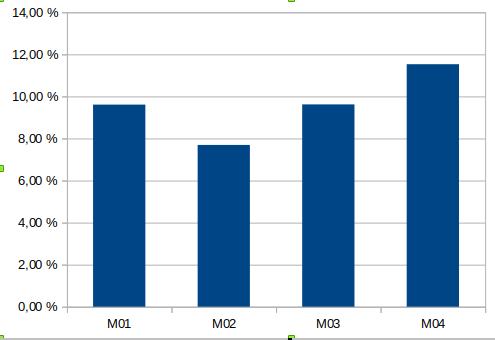
\includegraphics[]{corpus_bruite.png}
			\end{figure}
			//TODO expliquer le résultat.
		\subsubsection{Test 2.2: Corpus non-bruité}
			Dans cette section, nous avons le dossier référence les ordres $\in$ Ordre prononcés par F01, F02, F03, F04, F05, M01, M02, M03, M04, M05, M06, M07, M08, M09, M10, M11, M12 et M13.
			$Ordre = \{arrete_toi, atterissage, avance, decollage, droite, etatdurgence, faisunflip, gauche, plusbas, plushaut, recule, tourne_droite, tourne_gauche\}$
			\begin{table}
				\begin{tabular}{|c|c|}
					\hline
					& taux de reconnaissance \\
					\hline
					F01 & 9,40\% \\
					F02 & 7,26\% \\
					F03 & 7,69\% \\
					FO4 & 5,98\% \\
					F05 & 8,54\% \\
					M01 & 7,26\% \\
					M02 & 3,84\% \\
					M03 & 8,97\% \\
					M04 & 6,83\% \\
					M05 & 9,82\% \\
					M06 & 6,41\% \\
					M07 & 8,11\% \\
					M08 & 7,26\% \\
					M09 & 6,41\% \\
					M10 & 7,26\% \\
					M11 & 6,41\% \\
					M12 & 8,54\% \\
					M13 & 7,69\% \\
					\hline
				\end{tabular}
			\end{table}
		\subsubsection{Test 2.3: Enregistrements personnels}
		Dans cette section, nous avons dans le dossier reference les ordres $\in$ Ordre, prononcés par Ber, Gas, Lent, Nathan, Rapide, Tim, Vero.\\
		$Ordre = \{arrête toi, avance, fais un flip, gauche, droite, pendule inversé, recule, tourne droite, tourne gauche\}$
			\begin{table}[h]
				\begin{tabular}{|c|c|}
					\hline
					& taux de reconnaissance \\
					\hline
					Ber & 6.66\% \\
					Gas & 6.66\% \\
					Lent & 13.33\% \\
					Nathan & 17.7\% \\
					Rapide & 8.88\% \\
					Tim & 6.66\% \\
					Vero & 13.34\% \\
					\hline
				\end{tabular}
			\end{table}
			\begin{figure}[h]
   				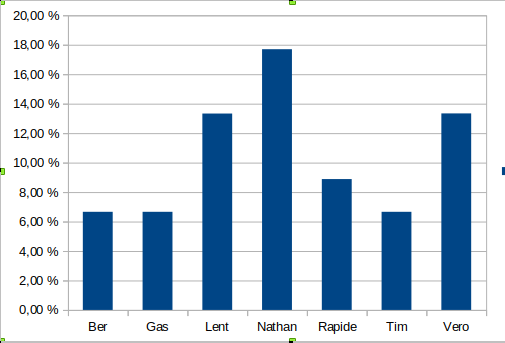
\includegraphics[]{enregistrement_perso.png}
			\end{figure}
			//TODO expliquer le résultat.

\end{document}